%=====================导=======言==============================
\documentclass[a4paper,11pt]{article}
%======================Include Packages========================

\usepackage[36428]{MCMthesis}  %队号在这里填写
%\usepackage[175,nosheet]{MCMthesis}%这个参数形式可去掉summary sheet首页。
\problem{B}  %选题
%===============设置正文和数学字体=============================
%有些字体需要安装一些字体文件,注意辨别。
%我参照 MCM论文集的字体 使用如下宏包来定制字体。
\usepackage{palatino}
\usepackage{longtable}

%设置段落之间的距离,若不需要删除或者注释掉即可。
\setlength\parskip{.5\baselineskip}

%def\abstractname{Summary}%可修改摘要名称

%%%%%%%%%%%%%%%%%%%%%%%%%%%%%%%%%%%%%%%%%%%%%%%%%%%%%%%%%%%%%%%%%%%
%%%%%%%%%%%%%%%%%%$$$$$$$==正文开始==$$$$$$$%%%%%%%%%%%%%%%%%%%%%%%
%%%%%%%%%%%%%%%%%%%%%%%%%%%%%%%%%%%%%%%%%%%%%%%%%%%%%%%%%%%%%%%%%%%

%==========================论文标题===============================
\title{An implement of film recommendation system based on statistical models}
\author{Team \#36428}
\date{\today}
%=================================================================
%==================================================================
\begin{document}
%摘要需要放在maketitle之前才能保证运行正常
%====================摘=======要===================================
\begin{abstract}
  With the rapid development in Internet technology, the trend of appreciating films online is becoming heated. In order to realize the maximum profits, it is essential for content providers to collect users' information, including both their basic personal identities and implicit  browsing histories and habits, to analyse their characteristic film styles and eventually recommend potential best choices for the users. Actually, this kind of application pipeline has been widely used like NetFlix[cite1], Hulu[cite2] and Amazon[cite3], etc. 
  In this competition problem, we are required to implement a simple version of such system. Therefore, we focus our attention on the utilization of raw data provided by MovieLens dataset[cite4] and model relatively precision and objective features for both users and movies. Later, we are able to analyse specific users'  film favor based on statistic approaches. In addition, with the aid of Support Vector Machine(SVM) and Classification and Regression Tree(C\&RT), we innovatively mine the implicit information from rating records and establish a predictive model based on users' and movies' features. Finally, we set experiments to compare our models with the traditional collaborative filtering algorithm and get some interesting conclusions. 
  
\begin{keywords}
recommendation system; collaborative filtering; SVM regression; C\&RT
\end{keywords}
\end{abstract}

\maketitle
\pagestyle{empty}
%
\newpage                                                          %
%==================================================================


%====================生=成=目=录===================================
\tableofcontents                                                  %                                            %
\newpage
\pagestyle{fancy}                                                     %
%==================================================================
%======================问题介绍====================================
\section{Introduction}
According to the statistical data collected by World Heath Organization(WHO)\cite{ebolafactsheet}, the current Ebola virus disease (EVD) outbreak ravaging three nations in West Africa has affected more than 14,000 persons and killed over 5,000. It is the longest and most widely spread Ebola epidemic ever seen.

In this problem, a new medication has just been released by the world medical association. We are required to undertake the duty of fight against the Azrael with the aid of this medicine: establishing a realistic sensible and useful model that consider various factors including spread speed, medicine manufacturing speed, delivery system, etc. In order to accomplish such a huge task, we establish two sub-models:

\begin{itemize}
\item \textbf{Sub-model 1:}A model which describes the virus dispersal process in ideal settings.
\item \textbf{Sub-model 2:}A model contains the deep relationship between the medication manufacturing, delivery, applying flow and the infection, immune process of EVD. 
\end{itemize} 

In sub-model 1, we implement a real-time simulation system by Matlab to simulate the dispersal process of Ebola in ideal cases. We modify the\textbf{ SIR} model into our \textbf{SID} one and exhibit you with touchable and vivid figures.

In sub-model 2, by surveying a large amount of real data, scientific paper available, we propose an all new model: \textbf{SPARD}, which takes not only: spread speed, harmfulness, delivery system, but also: manufacturing speed, dispersal path as essential factors into consideration. In addition, all these factors in \textbf{SPARD} model are dynamic changing and they provide us with a warning system which can aid us finding the trend of EVD dispersal as soon as possible.

The structure of the paper is organized by two sub-models, respectively. In each sub-model, we give our own analysis, assumptions, models descriptions, experiment results and strengths/weaknesses analysis. The final conclusion is given in section 4. In section 5, we provide our non-technical letter intended for world citizens. The appendix offers the raw data of our \textbf{SPARD} model.

\section{Sub-model 1: SID-The dispersal of the Azrael in ideal cases}
\subsection{Symbols and Notations}
\begin{table}[htbp]
\centering
\caption{Major Symbol and Notation list for sub-model 1}
 % Table generated by Excel2LaTeX from sheet 'Sheet1'
\begin{tabular}{|c|c|c|c|c|c|c|}
\hline
                                      \multicolumn{ 7}{|c|}{{\bf Symbols and Notations}} \\
\hline
\multicolumn{ 2}{|c|}{{\bf Symbol/Notation}} &                  \multicolumn{ 5}{|c|}{{\bf Definition}} \\
\hline
\multicolumn{ 2}{|c|}{$\tau$} & \multicolumn{ 5}{|c|}{The transmission probability from susceptible to infective} \\
\hline
\multicolumn{ 2}{|c|}{$\mu$} & \multicolumn{ 5}{|c|}{The transmission probability from infective to death} \\
\hline
\multicolumn{ 2}{|c|}{$S(t)$} & \multicolumn{ 5}{|c|}{The number of susceptible people at time t} \\
\hline
\multicolumn{ 2}{|c|}{$I(t)$} & \multicolumn{ 5}{|c|}{The number of infected people at time t} \\
\hline
\multicolumn{ 2}{|c|}{$D(t)$} &     \multicolumn{ 5}{|c|}{The number of dead people at time t} \\
\hline
\multicolumn{ 2}{|c|}{N} & \multicolumn{ 5}{|c|}{The total population in one district(default: 1 unit)} \\
\hline
\multicolumn{ 2}{|c|}{$t_{max}$} &                 \multicolumn{ 5}{|c|}{Maximum simulation days} \\
\hline
\multicolumn{ 2}{|c|}{$k$} &    \multicolumn{ 5}{|c|}{Average days to death after infected} \\
\hline
\end{tabular}  

\end{table}
\subsection{Analysis and Assumptions}
In this section, our goal is to construct a model which can provide us with a direct and visible Ebola spread process in those highlighted areas, specifically without any sanitation interference. The goal for constructing such an primary model is to set up a fundamental pipeline for further models, which introduced in the third sections. According to the official document, Guidance for Immunization Programmes in the African Region\cite{ebolaguide}, released in Oct. 2014, at the present EVD outbreak, the top three countries in EVD crisis, which means they own the most detected cases and fatality rates, are \textit{Guinea, Liberia and Sierra Leone}. Besides, \textit{Cote d' Ivorie, Guinea Bissau, Mali} and another eleven countries are in high infection risk. Just as we shown in \textbf{figure 1}, those countries are mostly in Western African regions.

In addition, according to another technical report\cite{team2014ebola} the common approach of EVD's spread are: human direct contacts, body fluid exchange, inappropriate bury, etc. One of the issues worthy noting is that no evidence yet attests that there exists human-stock dispersal path or ocean movement dispersal path. In other words, the spread of EVD major relies on high population density and commences from those inner parts of the continent. These facts imply that our EVD dispersal spread point in the simulation should be set in metropolitans. 
\begin{figure}[htbp]
\centering
\includegraphics[width=15cm]{/figure/fig1.jpg}
\caption{The present status of Ebola in Western African areas, according to WHO website} \label{fig:1}
\end{figure}
Besides, in order to direct observe the disastrous effect of Ebola and utilize the classical \textbf{SIR} model, we survey the Ebola's infection probability for a given patient from \cite{world2014ebola}. For simplification purpose, we utilize the "max-pooling" strategy to select our infectious probability $\tau$. And because we assume there does not exist any health or medication care system, we set the death rate $\mu$ as $100\%$ for those infected  inhabitants. Finally, due to the fact that the incubation period for an EVD patient ranges from 2-21 days\cite{wool1998characterization}, we suppose that the life-span only depends on the average incubation period.

On the basis of the analysis above, we summarize our assumptions as below:
\begin{itemize}
\item \textbf{Assumption 1-1:} The starting points of the dispersal should be those medium or big size cities rather than other points on the map.
\item \textbf{Assumption 1-2:} There is not any human medical-care action to impede or stop Ebola's spread. As long as someone is infected by EVD, he or she is bounded to death, i.e., $\mu=100\%$.
\item\textbf{Assumption 1-3:} The dispersal approach only includes continent-adjacent dispersal way.
\item\textbf{Assumption 1-4:} The lifespan for an infected people $k$ is a constant depending on the incubation period. In this case, $k=13$.
\end{itemize} 
\subsection{Model Description}
In this subsection, we briefly introduce the classical \textbf{S}usceptible, \textbf{I}nfective, \textbf{R}emoval(\textbf{SIR}) model\cite{mccluskey2010complete} in epidemic dynamic fields and our modification work on it. Besides, we will introduce the input parameters, output parameters and the basic flow of our simulation system.

First and foremost, according to the \textbf{SIR} model, as long as a particular region is affected by the Ebola, the whole population can be divided into three separate parts: \textbf{S}usceptible(People who are still in healthy status); \textbf{I}nfective(People who have already caught the EVD); \textbf{R}emoval (\textbf{SIR})(People who have already recovered and is immune to EVD). Nonetheless, on the basis on \textbf{Assumption 1-2}, there should not be any recovered  inhabitants. When we recall the fact that no matter recovered or death people are immune to the disease and are not able to further affect susceptible individuals. We can simply consider that "Removal" is equivalent to "Death"; therfore, we can modify \textbf{SIR} into \textbf{SID(death)} by setting D's immune index at 0(because they have already died). In addition, we assume that D class people are immediately buried appropriately after death.

Furthermore, the core part of the \textbf{SID} model can be described with two transmission probabilities: susceptible-infective: $\tau$ and infective-death:$\mu$. Based on our early premises, $\mu$ has already selected at $100\%$. As  to calculating susceptible-infective transmission probability $\tau$, we utilize the apex value in \cite{rebaudet2015ebola}, just as shown in \textbf{figure 2}. Therefore, we set $\tau$ at $0.4$.

\begin{figure}[htbp]
\centering
\includegraphics[width=15cm]{/figure/fig2.pdf}
\caption{The probability of infecting suspicible people of an EVD patient, with respect to time}\label{fig:2}
\end{figure}
According to \textbf{Assumption 1-4}, the lifespan for infected people $k=13 days$. 
Finally, The behaviour of our \textbf{SID} model can be described by a group of differential equations as below:
\begin{equation}
 \left\{
\begin{aligned}
S\left( t\right) +I\left( t\right) +D\left( t\right) =N \\
\dfrac {dS}{dt}=-\tau SI \\
\dfrac {dI}{dt}=\tau SI-I\mu \\
\dfrac {dD}{dt}=I\mu \\
S(0)=N, I(0)=0, D(0)=0
\end{aligned}
\right.
\end{equation}

Note that $N$ is the total population of a specific district; at the initial state, all the  inhabitants in one district are uninfected by EVD; and of course, there is no death. Thus, we set the initial value of the differential equation groups at $S(0)=N, I(0)=0, D(0)=0$.

The second task of this model is to determine other essential rules and parameters for our simulation system. Due to \textbf{Assumption 1-1}, we set the dispersal rule "four-adjacent" principle respect to the pixels on the map,i.e., if one particular pixel is set as infected status at day $n$, its four neighbour pixels(upper, lower, left and right one) have probability $\tau$ to be affected. Moreover, for the sake of observing the dynamic process of EVD's spread, we trace $t_{max}=120days$ to generate the simulation results. The evaluation metric is the relative ratio of S, I and D. Another interesting issue is to determine the starting cities of EVD in the simulation. \textbf{Assumption 1-1} and the characteristic of Ebola hint us to select those cities with large population and relatively lower hygiene level(although there is no heath care interference in this model). Therefore, we survey those potential cities with high EVD risk from WHO annual report\cite{worldworld}: a comprehensive evaluation between population and countries' hygiene level(hospital beds, physician numbers, etc). and eventually select four cities. Our investigation result about those cities is shown in \textbf{table 2}.
\begin{table}[htbp]
\centering
\caption{The survey result of four selected cities(data from WHO health statistic 2013)}
% Table generated by Excel2LaTeX from sheet 'Sheet1'
\begin{tabular}{|r|r|r|r|r|}
\hline
{\bf city} & {\bf country} & {\bf city population} & {\bf hospital beds\tnote{1}} & {\bf physician number\tnote{2}} \\
% city &  country &  city population & hospital beds\tnote{1} &  physician number \\
\hline
   Korhogo & Côte d'Ivoire &     174000 &        1.7 &        1.4 \\
\hline
    Kankan &     Guinea &     193830 &        1.2 &        0.9 \\
\hline
    Bamako &       Mali &    1800000 &        0.8 &          1 \\
\hline
    Tamale &      Ghana &     562919 &          1 &          2 \\
\hline
\end{tabular}  
\begin{tablenotes}
        \footnotesize
        \item[1] Remark: hospital beds and physician number are in 10,000 population scale.
\end{tablenotes}

\end{table}


\subsection{Experiment Result}
In this subsection, we exhibit the automatic simulation results of EVD in ideal cases. In \textbf{figure 3}, we show the relative S, I, D changing curve with respect to time:

\begin{figure}[htbp]
\centering
\includegraphics[width=15cm]{/figure/fig3.eps}
\caption{The S,I and D changing curve with respect to time}\label{fig:3}
\end{figure}

From the simulation figure, we can observe that the susceptible and death curve are changing exponentially. If we choose 80\% as the threshold of susceptible, a commonly used index to indicate the harmfulness of one particular pestilence, the milestone happens approximately on the 60th day. The counterpart index of SARS is 64th day\cite{small2006super}. Besides, in the light of the end part of the curve, we can predict that the percentage of death will exceed the percentage of susceptible in the following few days, which means the  "collapse" in this area. These facts notifies us that the Ebola is indeed a lethal disease with high infectious rate.
In \textbf{figure 4}, we visualize the dispersal process by sampling four days simulation results.
\begin{figure}[htbp]
\centering
\includegraphics[width=12cm]{/figure/fig4.pdf}
\caption{A dynamic dispersial process of EVD by sampling 1st day, 40th day, 80thday and 120th day}\label{fig:4}
\end{figure}
In \textbf{figure 4}, the continent parts with original color are uninfected areas(the S area); the pink parts are those districts which have already in collapse condition(the D area); the red outer skirt of the pink parts are districts where are suffering from the EVD(the I area). \textbf{Figure 4} inspire us at least in two aspects: 1. the dispersal of Ebola in ideal cases is a diamond-shape infiltration process(this can help us to predict risky districts); 2. As long as several infection districts are connected together, the red outer skirt will dramatically decrease, which means acute increase in death(therefore, we should stop this circumstance from happening).
\subsection{Strengths and Weaknesses}
\begin{itemize}
  \item Strenghs
  \begin{itemize}
    \item We successfully model the dispersal process of Ebola with revising the classical \textbf{SIR} model into \textbf{SID} model and by setting reality parameters to it.
    \item By utilizing the simulation system, there is no need to calculate the numerical solution of the differential equation group in \textbf{SID} model.
    \item The simulation system enables us to visualize the process of dispersal in a direct and human understandable way.
  \end{itemize}
  \item Weaknesses
  \begin{itemize}
    \item The primary model fails to evaluate some crucial factors which can affect the spread, for instance, there should be a relationship between the population density and the infection probability $\tau$ in a specific region.
    \item The simulation process itself may take a considerable time. In fact, we spend over three minutes to fetch the results on a Core-i5 PC with 8GB RAM. Apparently, both of the time and space consumptions are $O(mapSize*t_{max})$.
  \end{itemize}
\end{itemize}

\section{Sub-model 2: SPARD-Improved EVD dynamic dispersal model}
\subsection{Symbols and Notations}
\begin{table}[htbp]
\caption{Major Symbol and Notation list for sub-model 2}
\center
% Table generated by Excel2LaTeX from sheet 'Sheet1'
\begin{tabular}{|cc|ccccc|}
\hline
                                      \multicolumn{ 7}{|c|}{{\bf Symbols and Notations}} \\
\hline
\multicolumn{ 2}{|c|}{{\bf Symbol/Notation}} &                  \multicolumn{ 5}{|c|}{{\bf Definition}} \\
\hline
\multicolumn{ 2}{|c|}{$S(x,y,t)$} & \multicolumn{ 5}{|c|}{The number of susceptible people at time t} \\
\hline
\multicolumn{ 2}{|c|}{$P(x,y,t)$} & \multicolumn{ 5}{|c|}{The number of primary infected people at time t} \\
\hline
\multicolumn{ 2}{|c|}{$A(x,y,t)$} & \multicolumn{ 5}{|c|}{The number of advanced infected people at time t} \\
\hline
\multicolumn{ 2}{|c|}{$R(x,y,t)$} & \multicolumn{ 5}{|c|}{The number of recovered people at time t} \\
\hline
\multicolumn{ 2}{|c}{$D(x,y,t)$} &      \multicolumn{ 5}{|c|}{The number of dead people at time t} \\
\hline
\multicolumn{ 2}{|c|}{$N(x,y,t)$} & \multicolumn{ 5}{|c|}{The total population in one district(default: 1 unit)} \\
\hline
\multicolumn{ 2}{|c|}{$\tau(x,y,t)$} & \multicolumn{ 5}{|c|}{The transmission probability from susceptible to primary infected} \\
\hline
\multicolumn{ 2}{|c|}{$\mu(x,y,t)$} & \multicolumn{ 5}{|c|}{The transmission probability from advanced infected to death} \\
\hline
\multicolumn{ 2}{|c|}{$\lambda(x,y,t)$} & \multicolumn{ 5}{|c|}{The transmission probability from primary infected to recovery} \\
\hline
\multicolumn{ 2}{|c|}{$\eta(x,y,t)$} & \multicolumn{ 5}{|c|}{The transmission probability from susceptible to immune} \\
\hline
\multicolumn{ 2}{|c|}{$\phi(x,y,t)$} & \multicolumn{ 5}{|c|}{The transmission probability from primary infected to advanced} \\
\hline
\multicolumn{ 2}{|c|}{$t_{max}$} &                 \multicolumn{ 5}{|c|}{Maximum simulation days} \\
\hline
\end{tabular}  
\end{table}
\subsection{Analysis and Assumptions}
In this section, we concentrate our attention on further revising the simple \textbf{SID} model mentioned in the former section and improving the accuracy,  performance of our own model. Our contributions can be classified into four aspects:

\begin{itemize}
  \item The residents in one particular district $(x,y)$ at time $t$ is detailed divided into five categories: susceptible, primary infected, advanced infected, recovered and immune, death. All the values of these categories are variables with respect to spatial and temporal.
  \item We succeed in establishing a numerical relationship between transmission probabilities and the real-time number of five classes above. Thus, the probabilities themselves are also in dynamic status corresponding to time and geography location.
  
  \item We succeed in establishing the demand of the medication at $(x,y,t)$ dynamically, and construct an "\textbf{E}arly \textbf{W}arning \textbf{S}ystem(\textbf{EWS})" for vaccine actions.
  
  \item In the aspect of delivery system, we take the advantage of graph optimization technique to implement a optimized medication delivering  arrangement based on the dynamic actual demands.
  
 \end{itemize}
 
 The general human classification and their transmission probabilities is shown in \textbf{figure 5}. For abbreviation purpose, we name our model as \textbf{S}usceptible, \textbf{P}rimary, \textbf{A}dvanced, \textbf{R}ecovery, \textbf{D}eath(\textbf{SPARD}).
 
\begin{figure}[htbp]
\centering
\includegraphics[width=12cm]{/figure/fig5.pdf}
\caption{The five categories and their relationships of our proposed SPARD dispersal model}\label{fig:5}
\end{figure}

Our definition of "Susceptible", "Death" is as same as those in section 2: the primary \textbf{SID} model in ideal cases. What needs to be specially explained is: "Primary" status, people who have determined to have infected by EVD but still in primary stage. In other words, this kind of  inhabitants are treatable with the aid of our newly invented medication with probability $\lambda$. The counterpart of "P" status is "A": advanced infected status. People in this stage are unfortunately incurable by our medicine(because the problem says that the medicine is only valid to early stage people) and they are bounded to death at a constant rate. The transition probability from "P" stage to "A" stage is $\phi$. Moreover, thanks to the invention of vaccine by the world medication organization, people in susceptible status are able to become permanent immune to EVD(the "R" status) with probability $\eta$. 

Besides, in order to further simulate and analysis this model numerically , we put out following model premises. Note that some of them will be explained in detail in next subsections.

\begin{itemize}
\item \textbf{Assumption 2-1} There is no possibility of natural recovery for any EVD patient, no matter a primary stage one or an advanced stage one.
\item \textbf{Assumption 2-2} The effect of EVD dispersal at a specific point to its neighbourhood is a circle with constant radius, which modulated by a function. 
\item \textbf{Assumption 2-3} The dispersal abilities of "P" and "A" status patients are different constants.
\item \textbf{Assumption 2-4} A "P" status patient is usually with slight symptoms and is taken care by five families members(on average) every day. An "A" status patient is looked after by one professional medical staff(on average) during rest lifespan.
\item \textbf{Assumption 2-5} The medical level and  inhabitants' awareness to EVD is a monotonous increase function with respect to time.\cite{worldebola}
\item \textbf{Assumption 2-6} The average delivery period of both vaccine and remedial drug is a constant.
\end{itemize} 

\subsection{Model Description}
\subsubsection{General Model}
We get inspired from our primary sub-model 1 and \cite{shulgin1998pulse}. With the aid of flow chart shown in \textbf{figure 5}, the overall EVD dispersal system in district $(x,y)$ at time $t$ is still described by differential equation group as below:

\begin{equation}
 \left\{
\begin{aligned}
 S\left( x,y,t+1\right) =\left( 1-\tau -\eta \right) S\left( x,y,t\right) \\
 P\left( x,y,t+1\right) =(1-\phi-\lambda)p\left( x,y,t\right) +\tau S\left( x,y,t\right) \\
 A\left( x,y,t+1\right) =\left( 1-\mu \right) A\left( x,y,t\right) +\varphi P\left( x,y,t\right) \\
D\left( x,y,t+1\right) =D\left( x,y,t\right) +\mu A\left( x,y,t\right) \\
R\left( x,y,t+1\right) =R\left(x,y,t\right)+\lambda P\left( x,y,t\right) +\eta S\left( x,y,t\right) \\
\end{aligned}
\right.
\end{equation}

The differential equation group above describes the dynamic transition process from time $t$ to time $t+1$. Nonetheless, as mentioned in last subsection, in \textbf{SPARD}, the transition probabilities themselves are also dynamic. In other words, their values depend on the present status of a local point. From 3.3.2 to 3.3.7, we explain our models on these transition probabilities, respectively. In 3.3.8, we will introduce our \textbf{E}arly \textbf{W}arning \textbf{S}ystem(\textbf{EWS}) in detail. Section 3.3.9 is another graph optimization  model concerning transport optimization issue.

\subsubsection{Objective Condition Model}
According to the guide released intended to helping people fighting against EVD\cite{gradon2000outbreak}, it is highlighted that the hygiene infrastructure level, including hospital beds, laboratories and surveillance ability, along with local  inhabitants' awareness to EVD, play crucial roles in eradicating Ebola. In our SPARD model, we generally classify those factors as "Objective Conditions". As far as we are concerned, those objective conditions can be considered as an monotonous increase function to time, which means that the overall hygiene level and human beings knowledge to EVD is turning better daily(\textbf{Assumption 2-5}). 

To exemplifier this idea, we collect NGO volunteer number(data from \cite{nyenswah2014ebola,adraebola,emergencyebola}) and Isolation beds(data from \cite{adraebola,emergencyebola}) in Liberia as crucial hygienic index provided by WHO from March, 2013 to December, 2014, as shown in \textbf{Table 4}. The visualized curve figure is shown in \textbf{figure 6}.
\begin{table}[htbp]
\centering
\caption{NGO volunteer number and EVD isolation beds in Liberia} 
% Table generated by Excel2LaTeX from sheet 'Sheet1'
\begin{tabular}{|c|c|c|}
\hline
{\bf Date \tnote{1}} & {\bf NGO Volunteer Number \tnote{2}} & {\bf Isolated Beds} \\
\hline
    Mar-13 &        287 &        2.3 \\
\hline
    Jun-13 &        296 &        2.6 \\
\hline
    Sep-13 &        311 &        3.1 \\
\hline
    Dec-13 &        363 &        3.4 \\
\hline
    Mar-14 &        533 &       3.41 \\
\hline
    Jun-14 &        611 &        3.7 \\
\hline
    Sep-14 &        642 &          4 \\
\hline
    Dec-14 &        684 &        4.2 \\
\hline
\end{tabular}  
\begin{tablenotes}
        \footnotesize
        \item[1] Remark 1: NGO volunteer number is collected on: http://www.arda.org
        \item[2] Remark 2: Isolated beds number is in 10,000 population scale. collected from: http://www.emergency.it 
\end{tablenotes}

\end{table}

\begin{figure}[htbp]
\centering
\includegraphics[width=12cm]{/figure/fig6.pdf}
\caption{The visualized changing curve of NGO volunteer number and isolated beds number from Mar, 2013 to Dec, 2014}\label{fig:6}
\end{figure}

From \textbf{figure 6}, we can find that both the volunteer number and the number of isolation ward have always been increasing since March, 2013. In our opinion, the objective conditions level can be described with a logistic function\cite{dowell1999transmission} in order to reflect the process of relieving the effect of EVD dispersal resulted form objective conditions. Compared with \textbf{figure 6}, it is also reasonable to do so from the angle of functional fitting. Therefore, we define "Objective Condition Index" as below:

\begin{equation}
OCI\left( x,y,t\right) =\dfrac {1}{1+e^{-\dfrac{t}{30}}}
\end{equation}

What is amazing is that the shape of logistic function fits the blue curve(NGO volunteer number) quite well! This function implies that the $OCI$ can be viewed as a "discount"(range from 0-1) over the transition probability between a slight case to a severe one(S-P, P-A, etc).

\subsubsection{S-P Transition Model}
As far as we are concerned, the susceptible-primary stage transition probability is the core attribute to describe the EVD dispersal dynamic process, because it requires us to consider lots of inherent status of the location, i.e., the ratio among S, P, A, R, D people. First, we define the potential average number of an Ebola patient(both P and A types) can spread his or her virus, as the District Dispersal Index: $DDI$:

\begin{equation}
DDI=\dfrac {S}{S+R}\left({P}\times 5\times 23\% +{A}\times 1\times 81\% \right)\times OCI(x,y,t+1)
\end{equation}

$\dfrac {S}{S+R}$ is the ratio in healthy locals who can be infected by Ebola("S" people are not immune yet, whereas "R" ones are immune). Due to \textbf{Assumption 2-3}, we investigate the fact\cite{mushengxue} that, a "P" status patient has 23\% probability to spread disease to others; the same value of a "A" status one is 81\%. Moreover, according to \textbf{Assumption 2-4}, we add five(average families members number per "P" patient) and one(average medical staff number per "A" patient) to the inner product terms, respectively. 
Generally speaking, the $DDI$ tells us how many susceptible people can be infected in a particular district without considering inter-district spread cases under present situation. Finally, we add the $OCI$ term, to simulate the effect of objective conditions.

In order to calculate the precise ratio of S-P transition probability, i.e., the $\tau(x,y,t+1)$, we need to take district $(x,y)$ neighbourhood into consideration. There is a fact that a relatively farther district $(x_{1},y_{1})$ has less dispersal impact on $(x,y)$ than a near one $(x_{2},y{2})$. We utilize a two dimension Gaussian function $Gau(x,y)$ to conduct a convolution integral with $DDI(x,y,t)$ on spatial scale:

\begin{equation}
 \left\{
\begin{aligned}
Gau\left( x,y\right) =\exp\left(-\left( \dfrac {x^{2}+y^{2}}{\sigma ^{2}}\right)\right)\\
\tau \left( x,y,t+1\right) =\textbf{conv}\left[ DDI\left( x,y,t\right) ,Gau\left( x,y\right) \right]\\
\end{aligned}
\right.
\end{equation}

Note that in $Gau(x,y)$, the deviation coefficient $\sigma$, is a parameter to control the degree of popular density at neighbourhood around district $(x,y)$: imaging that for those metropolitan, $\sigma$ should be relatively large, because they have much stronger EVD radiation ability. \textbf{Figure 7} shows our settings of $Gau(x,y)$ for metropolitan($\sigma=250$), and normal villages($\sigma=150$), respectively.

\begin{figure}[htbp]
\centering
\includegraphics[width=15cm]{/figure/fig7.pdf}
\caption{The two dimension Gaussian function utilized to \textbf{conv} with DDI}\label{fig:7}
\end{figure}


\subsubsection{A-D Transition Model}
Unfortunately, the A-D transition ratio describes the process of advanced stage Ebola patient coming to death. In the light of an epidemic disease report \cite{dowell1999transmission} and our own investigation of the severe symptoms of advanced stage EVD patients(including fever, rash, vomiting, bleeding, etc), we give \textbf{Assumption 2-1} which means that the advanced EVD patients have no possibilities to recover and die at a fixed rate every day. We set this ratio at $20\%$. Thus, we have $\mu=0.2$.  

\subsubsection{P-A Transition Model}
Thanks to the improvement in objective condition: the increase of $OCI$ with respect to time, we consider the transition probability from primary EVD to advanced EVD $\phi(x,y,t)$ a constant multiplied by the updated $OCI$:
\begin{equation}
 \phi \left( x,y,t+1\right) =\phi \left( x,y,t\right) \times OCI(x,y,t+1)
\end{equation}

 \subsubsection{P-R Transition Model}
The P-R transition probability $\lambda$ means the ratio of  inhabitants, who have caught Ebola with slight symptoms, be cured on a particular day. According to our common sense, this index is an monotonous increase function with respect to time: the quality and performance of our newly invented medicine needs a process to be improved and become stable at last. This idea can be viewed as a simple deformation of \textbf{Assumption 2-5}. However, there is not any EVD-specific remedial medicine manufacturing data available yet. Thus, in order to attest our assumption, we cite the Yield-Time curve of the first counterpart for SARS, manufactured since Dec, 2004\cite{hensley2004interferon}. Then we conduct a regression analysis to achieve our $\lambda$ as shown in \textbf{figure 8}. 

\begin{figure}[htbp]
\centering
\includegraphics[width=15cm]{/figure/fig8.pdf}
\caption{The Yield-Time curve of remedial medicine for SARS, the regression result is used to describe our $\lambda$(Note that the temporal scale is month}\label{fig:8}
\end{figure}

We employee a logarithm function to regress the result. Therefore, our $\lambda$ is defined as:
\begin{equation}
\lambda \left( x,y,t+1\right) =0.195\ln \left( \dfrac{t}{30}\right) +0.35
\end{equation}

\subsubsection{S-R Transition Model}
The S-R transition probability $\eta(x,y,t)$ directly reflects the performance of vaccine medication. Apparently, for model simplification purpose, we utilize the \textbf{Assumption 2-5} like the P-R transition model again. However, the salient difference between P-R model and S-R model is that the speed of manufacturing a brand-new vaccine is much slower than that of remedial medicine. In this degree, the performance of the vaccine is determined as below by degrading the coefficients in some degree.
\begin{equation}
\eta \left( x,y,t+1\right) =0.080\ln \left( \dfrac{t}{30}\right) +0.1
\end{equation}

\subsubsection{Medication Demand and EWS}
Just as mentioned in previous sections, in our \textbf{SPARD} dispersal model, the medication is divided into two classes: vaccine and remedial drug. The \textbf{EWS} is meant to dynamically telling people the reasonable medication amount according to the evaluation results and real-time attributes in a specific area.

In the aspect of remedial drug demand, the situation is relatively easy to understand. The core principal is "How many sick, how much drug". Combining with \textbf{Assumption 2-1}, we only need to concentrate our attention on treating the "P" state patients and the \textbf{potential patients} before the next drug delivery period $T$(\textbf{Assumption 2-6}). Because the transition probability at time $t$ is $\tau$, and we have susceptible  inhabitants $S(x,y,t)$, primary symptom people $P(x,y,t)$. We arrange the remedial drug amount by predicting there will be $\tau$ ratio people caught EVD in the next $T$ days. Thus, the demand for remedial drug $DEM_{r}(x,y,t)$ is given as below:
\begin{equation}
DEM_{r}(x,y,t)=S\left( x,y,t\right) \sum ^{T}_{i=0}\left( 1-\tau \right) ^{i}\tau 
\end{equation}
On the other hand, the vaccine plays an important role in controlling the trend of EVD dispersal by lowering the risk of  inhabitants in a specific region to get caught the Ebola, i.e., lowering the value of $\tau$ and increase the value of $\eta$. Nevertheless, as we have deduced in S-P transition model, the probability of catching a EVD is not noly determined by the intra-district factors, but the neighbourhood regions, as well. On the basis of this premise, we use the $DDI$ attribute and the "convolution integral" trick in S-P Transition Model again to calculate the demand for vaccine $DEM_{v}(x,y,t)$:
\begin{equation}
DEM_{v} \left( x,y,t\right) =\textbf{conv}\left[ DDI\left( x,y,t\right) ,F_{vacc}\left( x,y\right) \right]
\end{equation}

However, in this case, we abandon the classical two dimension Gaussian function  to conduct the convolution. Instead, we define $F_{vacc}\left( x,y\right) $ in polar coordinate as $F_{vacc}\left(\rho,\theta\right)$ as following:
\begin{equation}
F_{vacc}\left(\rho,\theta\right) =
\left\{
\begin{aligned}
\log _{\dfrac {e}{2}}\left( \dfrac {1}{4}\rho\right), 0<\rho<7 \\
2.6\left( \dfrac {e}{2}\right) ^{9-\rho}, \rho\geq7
\end{aligned}
\right.
\end{equation}
The corresponding figure of $F_{vacc}\left(x,y)\right)$ is shown in \textbf{figure 9}.
\begin{figure}[htbp]
\centering
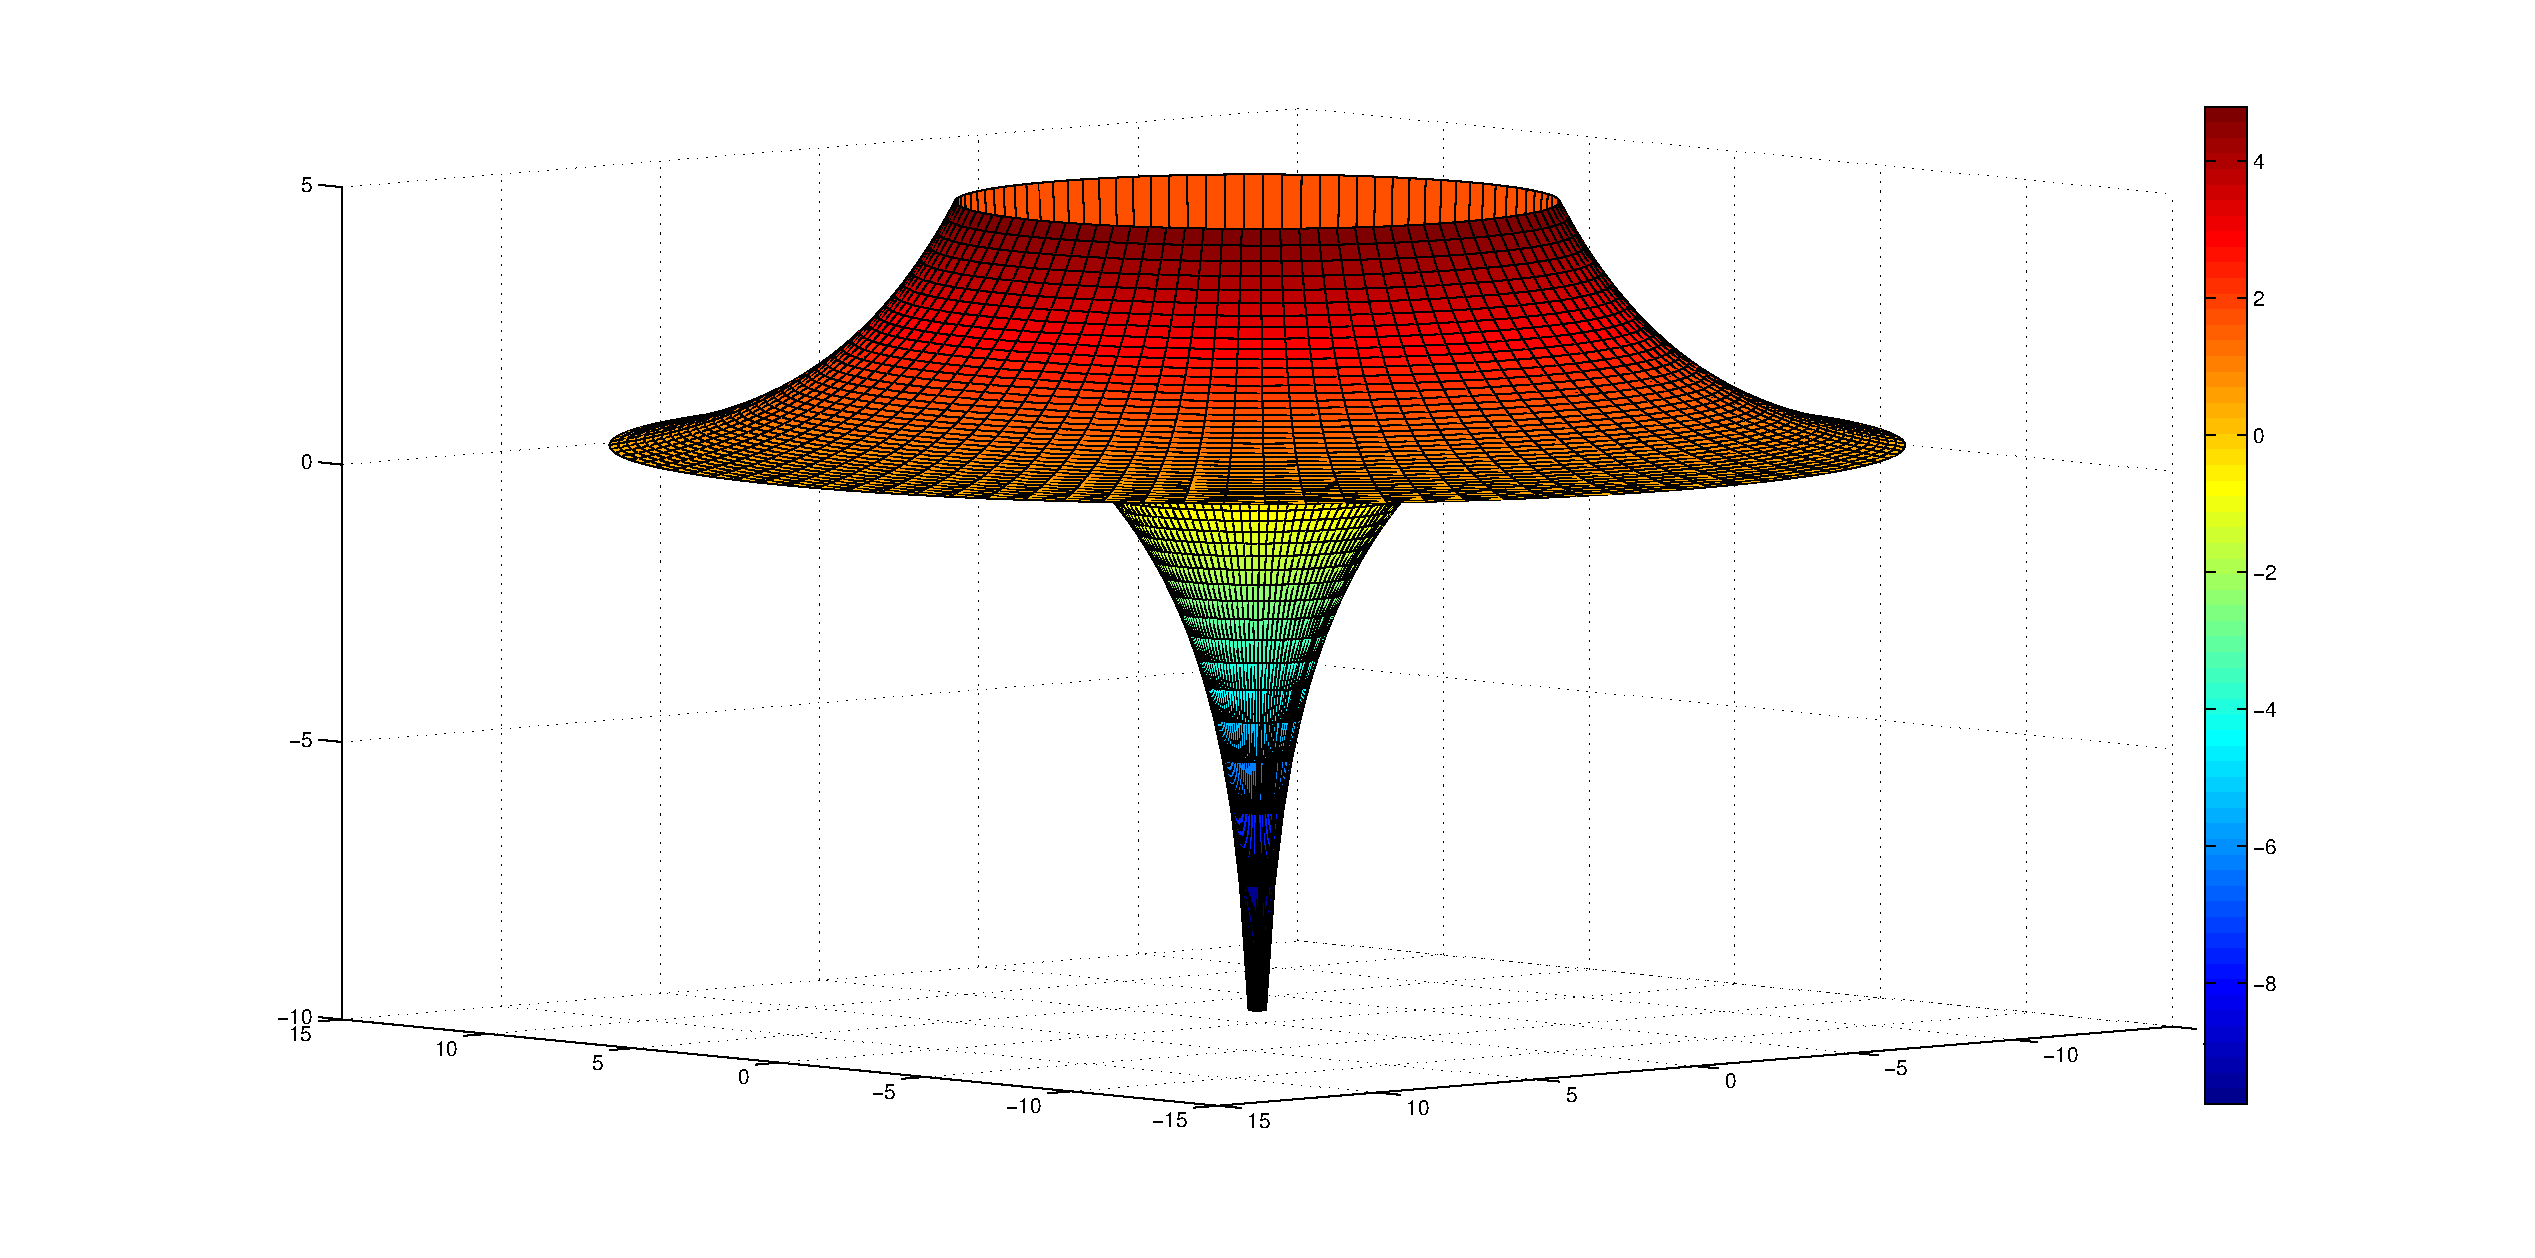
\includegraphics[width=15cm]{/figure/fig9.eps}
\caption{The 3D curve of our $F_{vacc}(x,y)$}\label{fig:9}
\end{figure}

Now, let us analysis the physical meaning and connection to \textbf{EWS} of this "weird" function. Given a specific severe infected region $(x,y)$, our goal is to prevent the process of EVD spread by arranging reasonable vaccine medication. We manually divide the neighbourhood of $(x,y)$ into two classes. 

The first classes includes those areas within a circle with radius at 7 unit length. Apparently, these areas are the most "dangerous" places , the absolute number of "P" status will sharply increase in a few days. Unfortunately, as you known, there always exists a "postpone" effect on the vaccine. In other words, it is too late to prevent EVD outbreak in these areas by distributing vaccine in short term. Actually, this action may even cause "excessive gathering" and panic among locals, as \cite{ungar1998hot} mentioned. This phenomenon explains why we set the nearest part(radius less than 7) around $(0,0)$ as negative. As to the second class parts, those areas with radius larger than the threshold 7, the vaccine should be monotonously decrease respect to distance, with the same purpose by employing Gaussian function in 3.3.4. This is just a crucial strategy in our \textbf{EWS}:"DO NOT waste vaccine resource on those most risky areas".

Overall, our \textbf{EWS} model designed for early warning and dynamic medication arrangement innovatively provides professions with direct and accurate real-time EVD dispersal evaluation metric. In addition, the authority can utilize \textbf{EWS} as an aid tool, to design daily transport plan.
 
\subsubsection{Transport Optimization}
In this section, we are meant to work out an optimized transport plan for the vaccine and remedial medicine. Because the expense of building a new airport will be considerable, our first mission is to minimize the total number of airports in the whole district. In order to simplify the task, we decompose the whole restrict into several hexagon subregions. Besides, we suppose that their is an small-scale size airport built for EVD in the middle of each hexagon. The idea to do so is inspired from the "cellular network" in Communication Engineering fields. Actually, this conclusion comes from \textbf{Theorem 3.1}.

\begin{Theorem} \label{thm:1}
    If we want to cover a plane with circles in same radius, when the circle center is the same as the gravity center of each hexagon in the hexagon grids, the total number of the circle in minimized.
\end{Theorem}

According to \textbf{Theroem 3.1}, we construct a cellular airport network as below:
\begin{figure}[htbp]
\centering
\includegraphics[width=13cm]{/figure/fig10.jpg}
\caption{The airport construction plan in western coast of Africa}\label{fig:10}
\end{figure}

In this way, we are able to cover the whole epidemic region with minimized airport number. The second task in our transport optimization model is to select several optimized airports as basements. In this task, we take the EVD dispersal situation every day into consideration. As mentioned in section 3.3.8, we have already defined the exact demand for remedial drug and vaccine as $DEM_{\tau}(x,y,t)$ and $DEM_{v}(x,y,t)$, respectively. Therefore, we can furthermore define a weight at each airport representing the "emergency degree for medication" for each hexagon region $R_{i}$:

\begin{equation}
 w_{i}=\iint_{R_{i}} \left( DEM_{\tau }\left( x,y\right) +DEM_{v}\left( x,y\right) \right) dR_{i}
\end{equation}

Then the task can be furthermore transfer into a graph optimization problem. Suppose we have $n$ airports with coordinates $(x_{j},y_{j}), j=1,2,...,n$, with weights $w_{j},j=1,2,3,...,n$. Our mission is to find $k$(the value depends on the general transport ability) basements $(x_{i},y_{i}), i=1,2,...,k$ {to minimize the following object function $L$, where $d_{ij}$ is the l2-norm between $(x_{i},y_{i})$ and $(x_{j},y_{j})$:

\begin{equation}
L=\sum _{i,j}w_{j}d_{ij}
\end{equation}

\begin{algorithm}[htbp] 
\caption{\small Finding the best $k$ basements by K-median point} 
\textbf{Input:} $w_{j}$, $(x_{j},y_{j})$, $j=1,2,...,n$ \\
\textbf{Output:} $(x_{qi},y_{qi})$, $i=1,2,...,k$ and $c_{ij}$ \\
\textbf{do}
\begin{enumerate} 
\item Randomly select $k$ points as  $(x_{qi},y_{qi})$. 
\item Group airports $(x_{j},y_{j})$ to the $k$ points by "minimize-distance" principle, i.e.: \\ 
  $c_{ij}=1$, where $d_{ij}=\min_{k}d_{kj}$. $c_{ij}$ is the adjacent matrix of the optimized graph.
\item Calculate the weighted geometry center in each airport group: $(x_{qi}',y_{qi}')$.
\item Calculate $L_{i}$ and $L'_{i}$ respectively, let $\varepsilon=\sum_{i=1}^{k}L_{i}-L'_{i}$.
\end{enumerate} 
\textbf{while} $\varepsilon$ not converge 
\label{alg1} 
\end{algorithm}

we solve this problem by the following \textbf{K-median point} algorithm in graph optimization theory as mentioned in \cite{har2005smaller}:

Thanks to the weight is calculated directly from the demand of medication, this optimized transport plan is coherently connected with our \textbf{EWS}. Thus, it can provide authority with a meaningful delivery suggestion.

\subsection{Experiment Result}
In the experiment section, we conduct the simulation experiment in two aspects. In the first part, in order to exhibit the transport optimization result, we sample one of the daily simulation result of the EVD dispersal and show our optimized plan in illustration form. In the second experiment, we verity the effect of our \textbf{SPARD} model and corresponding strategies by thoroughly comparing the simulation result under human interference condition with that without any medication supply(i.e., the ideal dispersal model).

First, let us verify our transport optimization model. We sample the $50th$ days' dispersal figure to deduce medication demand amount in one round of \textbf{SPARD} simulation under human interference conditions. \textbf{figure 11} is a coloured dynamic picture. The green regions are those areas which have majorly immune to EVD thanks to our \textbf{EWS} system. It is clear that in \textbf{figure 11}, there also includes a purple coloured stripe: the heated district where is suffering from EVD. Although there is another dark black sector(districts with people are almost all in "A" status), according to our principle in \textbf{EWS} model, the stripe area should be the on the top of our medication delivery list. 

\begin{figure}[htbp]
\centering
\includegraphics[width=15cm]{/figure/fig11.jpg}
\caption{The raw EVD dispersal figure on day 50}\label{fig:11}
\end{figure}

With the real-time value of $DEM_{\tau}(x,y)$ and $DEM_{v}(x,y)$ generated from our system,  we then calculate the weight $w_{i}$ for each hexagon region center(the values are shown in \textbf{figure 12} with red color). The real-time values of $w_{i}$ also reflect our guess in \textbf{EWS} in another way.

By conducting our \textbf{K-median point} algorithm, we eventually get the optimized transport plan under $k=3$. We label the airport selection plan with three different coloured lines in \textbf{figure 12}. In addition, we work out the homologous minimized object function value $L_{min}=1059$.

\begin{figure}[htbp]
\centering
\includegraphics[width=15cm]{/figure/fig12.jpg}
\caption{The corresponding optimized air basement arrangement of figure 11}
\end{figure}

Now it is time for us to overall evaluate the actual effect of \textbf{SPARD} with the classical \textbf{SID} model. Once again, we exhibit the evaluation result by vivid illustrations shown in \textbf{figure 13}.

\begin{figure}[htbp]
\centering
\includegraphics[width=17cm]{/figure/fig13.pdf}
\caption{The dynamic dispersal illustrations under SPARD framework with and without medication supply, respectively.}
\end{figure}

\begin{figure}[htbp]
\centering
\includegraphics[width=15cm]{/figure/fig14.pdf}
\caption{The S, P, A dynamic changing curve in SPARD with respect to time}
\end{figure}

In the left part of \textbf{figure 13}, we show the simulation results of EVD spread in ideal \textbf{SID} model on sampled days(10th day, 60th day, 90th day and 150th day). On the contrary, the right part shows the result of optimized \textbf{SPARD} model. In general, we represent the continent with cyan and the ocean with pure blue. Note that the dark purple part on the continent represents districts with residents majorly in "D" status, i.e, the terrify "collapse" caused by Ebola. Moreover, the green part is our vaccine covered area, with majorly R status people. Comparing with the simulation result of \textbf{SID}, our improved  \textbf{SPARD} model have the following apparent advantages:

\begin{itemize}
\item The simulation process itself is much more realistic. Both the left and right spread processes are no longer regular circles with gradually increasing radius.

\item Comparing the left figures with right ones, our core strategies in \textbf{SPARD} have salient performance on impeding Ebola death rate: the spaces of purple regions are all much smaller than the left ones.

\item The \textbf{EWS} mechanism also predicts the trend of EVD spread accurately: those green areas are exactly the spread directions in left figures.
\end{itemize}

In order to numerically compare the performance between \textbf{SPARD} with \textbf{SIR}, we plot the absolute number changing curves for S, P, A type residents in \textbf{figure 14}. The object region is the whole Western Africa continent. The strategies mentioned above give us with perfect performances in all three data curves: the susceptible cases number decrease much slower than that in \textbf{SID} settings, particularly after 100 days; the primary cases number in our model is kept stable throughout the whole simulation iterations; as to the advanced EVD patients number, thanks to the invention of the medication and our \textbf{EWS} action, the result is amazingly outstanding. Overall, the Azrael, Ebola is suspended by human beings after 200 days! Besides, the raw data in the iteration process is provided in Appendix.

\subsection{Strengths and Weaknesses}
\begin{itemize}
  \item Strenghs
  \begin{itemize}
    \item In our \textbf{SPARD} model, all parameters are dynamic changing with respect to the process of human being's fighting against  Ebola. Thus, we endow all the parameters in the model with touchable physical meanings. 
    \item We innovatively propose an early warning mechanism to impede the spread of Ebola. Governments and organizations can use the \textbf{EWS} to constitute scientific decisions.
    \item The \textbf{SPARD} model also provides a reasonable solution to the tricky medication delivery problem with the inspiration from modern communication systems.
  \end{itemize}
  \item Weaknesses
  \begin{itemize}
    \item Because of the time issue in this competition, some of the parameters in our model are lack of strict sensitivity analysis. Thus, some models may need further modification and tuning. 
    \item The simulation process itself takes a much longer time than sub-model 1 due to the great expansion in variables. We are even obliged to make use of a updated workstation to run our simulation program.
    \end{itemize}
\end{itemize}

\section{Conclusion}
In this paper, we establish two models to solve the problem concerning with eradicating the Azrael, Ebola. In model 1, we simply change the ordinary \textbf{SIR} model into \textbf{SID} by making some basic assumptions specific for observing Ebola's dispersal in ideal environments. The simulation result shows us an impressive spread ability of the lethal virus. Our attention is majorly concentrated on the second sub-model: \textbf{SPARD}. In this model, we design a dynamic process of the transition probabilities among those people classes. Therefore, the simulation result is much more precise and reasonable compared with the former one. Besides, the \textbf{SPARD} model also provides professions, governments and NGOs with an automatic early warning system, along with a complete solution plan to help fighting against EVD. Considering the fact that this MCM problem is not only challenging but also with practical senses, our team have decided to furthermore exploit the performance of our model. We plan to improve our model by using our knowledge in Machine Learning and Data Mining fields. For example, the simulation speed can be greatly improved by CUDA, a parallel calculation technology provided by NVIDIA \cite{nvidiacuda}. The up-to-date codes and models can be viewed at our Github page(E-mail us if needed).

\section{The non-technical letter}
Dear world citizens,

  We are pleased to announce our recent breakthrough in eradicating Ebola virus fields. After several years continuous dedicated work, our top-level research team has successfully manufactured the vaccine along with the medication which can impede the step of Ebola.
  
  As you known, at present, the lethal virus is raging on the western coast of the African continent. Every day, hundreds of our compatriots are suffering from the pain caused by Ebola. In fact, human beings are going through the toughest times to fight against the disease. 
  
  Therefore, for the humanitarian reasons, we have decided to provide our newly invented medicine and vaccine for free to those  inhabitants in high risk districts. According to a recent proposed paper concerning fighting against Ebola, the manufacturing speed of our medicine plays an crucial role in impeding its step. Thus, we are contacting closely with the best drug manufacturers at present in order to realize a stable and high quality production as soon as possible. Please trust us, there is no need to worry too much about the deadly disease. 
  
  Moreover, we have to remind you that every individual is an essential part on the frontline eradicating Ebola. As a worldwide health organization, we hope you to embrace the following personal habits to help us avoiding Ebola:

  \begin{itemize}
    \item Washing your hands and taking shower regularly as long as it permits;
    
    \item Avoiding visiting the epidemic area except you have professional protective equipments;
    
    \item Paying attention to the food you purchase, refuse those potential ingredients coming from the epidemic districts;
    
    \item Never hesitating to report to the local hygiene departments if you find yourself or friends have suspicious symptoms: fever, vomiting, rash, abnormal bleeding, etc;
    
    \item Keeping yourself updated with the dispersal news and prepare yourself if needed.
    
  \end{itemize}

With the corporation from all the human kinds, we believe that the Ebola will ultimately be eliminated in the near future. God bless you! God bless Africa!
\\
\\
Yours sincerely,

\textit{The World Medication Organization }
\newpage

\bibliography{cites}

\newpage
\begin{appendices}
\section{Raw data in \textbf{SPARD} model}
\subsection{Western African city data used in our simulation}
\begin{longtable}{|r|r|r|r|r|}
% Table generated by Excel2LaTeX from sheet 'Sheet1'
\caption{Western African city data}\\
\hline
{\bf city name} &    {\bf x} &    {\bf y} & {\bf population(1000)} & {\bf city size} \\
\hline
     Daker &         41 &         40 &        500 &      large \\
\hline
    Banjul &         51 &         72 &        500 &      large \\
\hline
    Bissau &         73 &        114 &        500 &      large \\
\hline
   Conakry &        151 &        183 &        500 &      large \\
\hline
  Freetown &        148 &        212 &        500 &      large \\
\hline
  Monrovia &        205 &        262 &        500 &      large \\
\hline
    Bamako &        280 &         96 &        500 &      large \\
\hline
Yamoussoukro &        350 &        248 &        500 &      large \\
\hline
Ouagadougou &        449 &        100 &        500 &      large \\
\hline
     Accra &        489 &        283 &        500 &      large \\
\hline
Saint-Louis &         53 &         15 &        375 &     medium \\
\hline
  Diourbel &         60 &         38 &        375 &     medium \\
\hline
   Kaolack &         50 &         52 &        375 &     medium \\
\hline
Serrekunda &         49 &         85 &        375 &     medium \\
\hline
Ziguinchor &         59 &        100 &        375 &     medium \\
\hline
     Kayes &        188 &         42 &        375 &     medium \\
\hline
    Kindia &        153 &        168 &        375 &     medium \\
\hline
    Kankan &        246 &        165 &        375 &     medium \\
\hline
     Koidu &        199 &        212 &        375 &     medium \\
\hline
    Kenema &        192 &        232 &        375 &     medium \\
\hline
       Man &        283 &        242 &        375 &     medium \\
\hline
   Korhogo &        343 &        176 &        375 &     medium \\
\hline
  Koutiala &        346 &        113 &        375 &     medium \\
\hline
     Mopti &        377 &         42 &        375 &     medium \\
\hline
     Segou &        325 &         72 &        375 &     medium \\
\hline
     Daloa &        322 &        250 &        375 &     medium \\
\hline
    Gagnoa &        351 &        263 &        375 &     medium \\
\hline
Abengourou &        395 &        246 &        375 &     medium \\
\hline
   Abidjan &        384 &        292 &        375 &     medium \\
\hline
 San-Pedro &        314 &        306 &        375 &     medium \\
\hline
    \multicolumn{ 5}{|l|}{{\bf *DO NOT include random cities}} \\
\hline
\end{longtable}

\subsection{Simulation raw data of S, P, A(sampled with 5 days interval}
% Table generated by Excel2LaTeX from sheet 'S'

\begin{longtable}{|>{\small}c|>{\small}c|>{\small}c|>{\small}c|>{\small}c|>{\small}c|>{\small}c|}
\caption{Simulation raw data of S, P, A(sampled with 5 days interval}\\
\hline
 {\bf day} & {\bf S(with med)} & {\bf S(without med)} & {\bf P(with med)} & {\bf P(without med)} & {\bf A(with med)} & {\bf A(without med)} \\
\hline
         5 &   14976623 &   14976369 &     252350 &     250705 &     108349 &     111075 \\
\hline
        10 &   14738090 &   14737688 &     242830 &     244329 &     194750 &     204560 \\
\hline
        15 &   14530769 &   14528287 &     215514 &     227892 &     201437 &     223864 \\
\hline
        20 &   14329028 &   14321353 &     195705 &     222019 &     183487 &     223662 \\
\hline
        25 &   14111004 &   14094203 &     185644 &     232828 &     169016 &     229464 \\
\hline
        30 &   13877055 &   13853705 &     176708 &     241358 &     159261 &     242268 \\
\hline
        35 &   13677715 &   13644777 &     134508 &     224921 &     133028 &     236912 \\
\hline
        40 &   13475748 &   13424671 &     105564 &     228296 &     101835 &     231394 \\
\hline
        45 &   13281873 &   13196534 &      84683 &     236752 &      77191 &     232168 \\
\hline
        50 &   13056665 &   12910363 &      91887 &     278823 &      64340 &     252104 \\
\hline
        55 &   12805749 &   12642965 &     108335 &     275748 &      64595 &     273871 \\
\hline
        60 &   12577016 &   12361087 &     102214 &     289777 &      60879 &     280214 \\
\hline
        65 &   12343194 &   12020161 &     101806 &     335642 &      51948 &     302659 \\
\hline
        70 &   12065897 &   11627542 &     129357 &     385074 &      52964 &     343366 \\
\hline
        75 &   11745289 &   11226831 &     178484 &     401485 &      72344 &     383971 \\
\hline
        80 &   11407989 &   10868984 &     227860 &     380513 &      99005 &     391497 \\
\hline
        85 &   11102780 &   10492122 &     235726 &     389367 &     113982 &     388249 \\
\hline
        90 &   10811852 &   10106981 &     221931 &     396813 &     112636 &     394796 \\
\hline
        95 &   10524957 &    9708419 &     211823 &     410794 &     106661 &     402641 \\
\hline
       100 &   10244242 &    9253499 &     208487 &     454814 &      99440 &     425921 \\
\hline
       105 &    9964654 &    8756677 &     204480 &     493391 &      95011 &     465931 \\
\hline
       110 &    9674931 &    8310848 &     207194 &     470739 &      95709 &     481452 \\
\hline
       115 &    9356791 &    7856101 &     231756 &     473636 &      98878 &     478255 \\
\hline
       120 &    9028581 &    7409922 &     263886 &     465844 &     102242 &     478702 \\
\hline
       125 &    8712221 &    6980690 &     280787 &     455296 &     104754 &     468732 \\
\hline
       130 &    8409114 &    6516381 &     281887 &     475411 &     107876 &     471968 \\
\hline
       135 &    8114938 &    6046523 &     274147 &     485033 &     107626 &     483124 \\
\hline
       140 &    7811628 &    5563885 &     271326 &     497476 &     106817 &     493312 \\
\hline
       145 &    7511821 &    5062757 &     269756 &     514337 &     108683 &     507369 \\
\hline
       150 &    7229198 &    4547124 &     252508 &     528814 &     107947 &     523439 \\
\hline
       155 &    6952562 &    4038297 &     231148 &     530155 &     103293 &     532049 \\
\hline
       160 &    6666080 &    3502737 &     217556 &     547673 &      99588 &     544252 \\
\hline
       165 &    6353021 &    3022293 &     228397 &     512139 &      95908 &     544043 \\
\hline
       170 &    6029395 &    2575120 &     249268 &     480538 &      95248 &     518447 \\
\hline
       175 &    5699390 &    2161231 &     270662 &     443396 &      98162 &     490278 \\
\hline
       180 &    5370738 &    1811827 &     288558 &     385364 &     100922 &     448661 \\
\hline
       185 &    5039376 &    1520986 &     309303 &     328427 &     106540 &     392406 \\
\hline
       190 &    4705252 &    1245123 &     323539 &     299157 &     116403 &     345440 \\
\hline
       195 &    4357208 &    1027669 &     343005 &     246405 &     128272 &     303391 \\
\hline
       200 &    4005844 &     854749 &     360557 &     201464 &     141712 &     253183 \\
\hline
       205 &    3650781 &     697349 &     377906 &     174591 &     151196 &     214176 \\
\hline
       210 &    3300298 &     562707 &     386778 &     151656 &     157306 &     181739 \\
\hline
       215 &    2977117 &     433580 &     368580 &     138406 &     161137 &     160864 \\
\hline
       220 &    2688953 &     334988 &     321209 &     112979 &     155327 &     140427 \\
\hline
       225 &    2424911 &     256396 &     270078 &      91397 &     142230 &     116611 \\
\hline
       230 &    2181498 &     193151 &     216114 &      73996 &     127091 &      95368 \\
\hline
\end{longtable}  


\end{appendices}


\end{document}
%%%%%%%%%%%%%%%%%%%%%%%%%%%%%%%%%%%%%%%%%%%%%%%%%%%%%%%%%%%%%%%%%%%
%%%%%%%%%%===========THE END OF PAPER============%%%%%%%%%%%%%%%%%%
%%%%%%%%%%%%%%%%%%%%%%%%%%%%%%%%%%%%%%%%%%%%%%%%%%%%%%%%%%%%%%%%%%%
